\documentclass[letterpaper]{jpconf}

\usepackage{url}                % For email addresses, hypertext links, ...
\usepackage{graphicx}
\usepackage{rotating}
\DeclareGraphicsExtensions{.pdf}
\setlength\topmargin{-.5in}

\begin{document}

\title{Interoperable Mesh Components For Large-Scale, Distributed-Memory Simulations}
\author{K. Devine$^1$, L. Diachin$^2$, J. Kraftcheck$^4$, 
        K. E. Jansen$^3$, V. Leung$^1$, X. Luo$^3$, M. Miller$^2$,
        C. Ollivier-Gooch$^5$, A. Ovcharenko$^3$, 
        O. Sahni$^3$, M. S. Shephard$^3$,
        T. Tautges$^6$, T. Xie$^3$, M. Zhou$^3$}
\address{$^1$ Sandia National Labs, Albuquerque, NM,
	 $^2$ Lawrence Livermore National Lab, Livermore, CA,
         $^3$ Rensselaer Polytechnic Institute, Troy, NY, 
         $^4$ University of Wisconsin, Madison, WI,
         $^5$ University of British Columbia, Vancouver, BC,
         $^6$ Argonne National Laboratory, Argonne, IL}
\ead{kddevin@sandia.gov, diachin2@llnl.gov, kraftche@cae.wisc.edu, jansen@rpi.edu, vjleung@sandia.gov, xluo@scorec.rpi.edu, miller86@llnl.gov, cfog@mech.ubc.ca, shurik@scorec.rpi.edu, osahni@scorec.rpi.edu, shephard@scorec.rpi.edu, tautges@mcs.anl.gov, txie@scorec.rpi.edu, zhou@scorec.rpi.edu}

\begin{abstract}
SciDAC applications have a demonstrated need for advanced software
tools to manage the complexities associated with sophisticated
geometry, mesh, and field manipulation tasks, particularly as computer
architectures move toward the petascale. In this paper, we describe a
software component --- an abstract data model and programming
interface --- designed to provide support for parallel unstructured
mesh operations.  We describe key issues that must be addressed to
successfully provide high-performance, distributed-memory unstructured
mesh services and highlight some recent research accomplishments in
developing new load balancing and MPI-based communication libraries
appropriate for leadership class computing.  Finally, we give examples
of the use of parallel adaptive mesh modification in two SciDAC
applications.
\end{abstract}

\section{Introduction}
\label{sec:intro}

Many simulations for solving partial differential equations (PDEs)
require the ability to model complex geometries defined by CAD or
other engineering design tools.  Such geometries in turn require 
the generation of meshes that have high fidelity to both
the computational domain description as well as to the features of
interest in the numerical solution, e.g., regions of high gradients.
This process is further complicated by the need to perform simulations
on petascale computers where additional issues such as load balance,
communication costs, and optimal data decompositions come into play.
Because these operations are common to many simulations, re-usable
software for these tasks can be shared across many application codes
which could reduce the time, effort, and expertise
required to develop and maintain simulation software.

Reuse of scientific software has traditionally relied on the use of
\emph{frameworks} or \emph{library-based} implementations and many
useful tools have been developed over the years for both unstructured
(e.g., \cite{ReSh03,Seol06,moab,GRUMMP:http,nwgrid3}) and structured
meshes (e.g., \cite{chombo,SAMRAI,overture}).  In addition, libraries
that provide mesh quality improvement
\cite{mesquite_download,frei-cfog:ijnme97}, front tracking
\cite{BoFi07}, mesh refinement \cite{LiSh05}, and parallel
partitioning and load balancing \cite{devi02} have been developed as well. 
However, the use of libraries or frameworks can significantly 
hamper experimentation with different software instances that provide
similar functionality.  In particular, libraries of similar purpose
often package functionality in very different ways. Consequently, data
structures shared between the application and library and even the
control flow between the application and library may need to be
totally re-designed.  This is especially true for meshing and geometry
libraries where applications often directly access the underlying data
structures, which can be quite different from implementation to
implementation.  Thus, using different libraries interchangeably or
interoperably for this functionality has proven difficult at best and
has hindered the wide spread use of advanced meshing and geometry
tools developed by the research community.

\emph{Components} represent a higher level of abstraction than libraries.
Essentially, a component defines both a \emph{specification} for an
application programming interface (API) and an abstract \emph{data
model} defining the semantics of the data that is passed through the
interface. There are several key advantages to using a component-based
approach in that the focus is on interfaces rather than on data
structures or file formats.  This allows any application using a
component to use another implementation of the same component API,
because all implementations have substantially equivalent
functionality.  
%Moreover, several strategies can be used to facilitate
%incremental adoption of components including the use of independent
%interfaces for distinct data model abstractions (e.g., one interface
%for the mesh and a separate interface for the geometry), the use of
%service-dependent interfaces to reduce the number of functions that
%need to be implemented and tested, and the finer granularity of the
%component interfaces reduces the need to mix huge libraries together.

In this paper, we describe a parallel unstructured mesh component
developed by the Interoperable Technologies for Advanced Petascale
Simulations (ITAPS) project (Section \ref{sec:component}).  As we have
worked to scale the software that uses our mesh component
implementations to 100,000 processors and beyond, several interesting
research projects to improve load balance and reduce communication
costs have arisen.  We briefly describe our work in these areas and
show both weak and strong scaling results for implicit finite
element/volume solvers and adaptive mesh refinement services (Section
\ref{sec:petascale}).  We conclude by showcasing the use of the
adaptive mesh refinement service in accelerator and fusion SciDAC
applications (Section \ref{sec:application}).

\section{The ITAPS Parallel Mesh Component}
\label{sec:component}

The ITAPS parallel mesh component builds on previous work that
resulted in the definition of a serial abstract data model and
interfaces for serial mesh data.  In this section, we briefly describe the
key concepts from that earlier work that are germaine to the current
discussion, and describe the parallel data model (Section
\ref{sec:data_model}) and language- and data-structure-independent
interface to support query and modification of meshes on distributed
memory computers (Section \ref{sec:interface}).  We then highlight
several software implementations of the interface and services that
use the serial and parallel interfaces to provide key functionality to
application codes (Section \ref{sec:software}).
 
\subsection{The Abstract Data Model}
\label{sec:data_model}

At a high level, the ITAPS data model divides the data required by a
simulation into three {\it core data types}: the geometric data, the
mesh data, and the field data.  These core data types are associated
with each other through {\it data relation managers}. The data
relation managers control the relationships among two or more of the
core data types, resolve cross references between entities in
different groups, and can provide additional functionality that
depends on multiple core data types.  Key building blocks within these
data models are the concepts of {\it entities}, {\it entity sets}, and
{\it tags}.
\begin{itemize}

\item {\it Entities} are used to represent atomic pieces of information
such as vertices in a mesh or edges in a geometric model.
Entity adjacency relationships define how the entities connect to
each other and both first-order and second-order adjacencies are
supported.

\item {\it Entity sets} are arbitrary collections of entities that may
be an ordered list or unordered.  The two primary supported
relationships among entity sets are {\it contained in} and {\it
parent/child} to allow for subsetting and hierarchical
applications. In addition, entity sets also have ``set operation''
capabilities such as set subtraction, intersection, or union.

\item {\it Tags} are used as containers to attach user-defined data to
ITAPS entities and entity sets.  Tags can be multi-valued which
implies that a given tag handle can be associated with many different
entities.  We support specialized tag types for improved performance
as well as the more general opaque case that allows any type of data
to be attached.
\end{itemize}
To support many of the services that applications desire, such as
adaptive mesh refinement, the data model includes the concept of
modification to allow changes to geometry, topology, or set structure.
In the case of the mesh, capabilities include changing vertex
coordinates and adding or deleting entities. Modification often
requires interactions between the mesh, geometry and field data models
and is one of the primary uses for the data relations manager.

The parallel ITAPS data model extends the concepts described above to
handle the requirements of distributed memory applications. In such
applications, the unstructured mesh is typically divided or {\it
partitioned} over the independent processor memories of the computer.
To be useful to applications, we must maintain information about mesh
entities and their adjacencies that is ``shared''.  In addition,
applications require the ability to move mesh entities and their
associated information between different processors to update the mesh
partition while maintaining this shared information.  Moreover,
applications expect that the mesh data model defined previously will
continue to work as expected within a process or for global address
spaces and shared memory paradigms.  These requirements are addressed
through the following additional core concepts.

\begin{itemize}

%\item A {\it process} is the executing program; often an MPI process.  
%The number processes is equal to {\tt MPI\_Comm\_size}, and the process
%number is equal to {\tt MPI\_Comm\_rank}.
%
\item A mesh {\it partition} is a decomposition of the mesh entities 
(e.g., vertices, edges, faces, and regions) into subsets called {\it
parts}.  The partition is responsible for mapping the entities to
parts and for mapping the parts to processes.  We note that each
process may have one or more parts and that each part is wholly
contained within a process.  Parts are identified globally by unique
part IDs and, within a process, by opaque part handles.  A partition
has a communicator associated with it.  Thus ``global'' operations are
performed with respect to data in all parts in the partition's
communicator and ``local'' operations are performed with respect to
either a part's or process's data.

\item Mesh entities are {\it owned} by exactly one part in the
partition where ownership imbues the right to modify. It is important
to note that ownership is not necessarily static during the course of
a computation and can be changed due to a repartitioning of the mesh
or due to local micro-migration operations.  In addition, some
entities will have read-only copies on other parts, for example, along
part boundaries and for ghosting operations. No globally unique
entity IDs are required or supplied by the data model although they can be
constructed by the user as a pair {\it [part ID, entity handle]}.

\item Mesh entities can be further classified as an {\it internal entity} (an owned
entity not on an interpart boundary), {\it a part-boundary entity} (an
entity on an interpart boundary which are shared between parts), or a
{\it ghost entity} ( a non-owned, non-part-boundary entity); see
Figure \ref{fig:data_model}. {\it Copies} are defined to be all ghost
entities plus all non-owned part-boundary entities.  The data model
defines rules for the amount of information about copies that an
implementation must manage.  For example, an entity's owner must store
information about all copies of the entity, and a copy must store
information about the entity's owner.  Remote parts and entities are
computed after mesh modification so
that queries for remote data do not require communication.

\end{itemize}

\begin{figure}[htb] 
\begin{center}
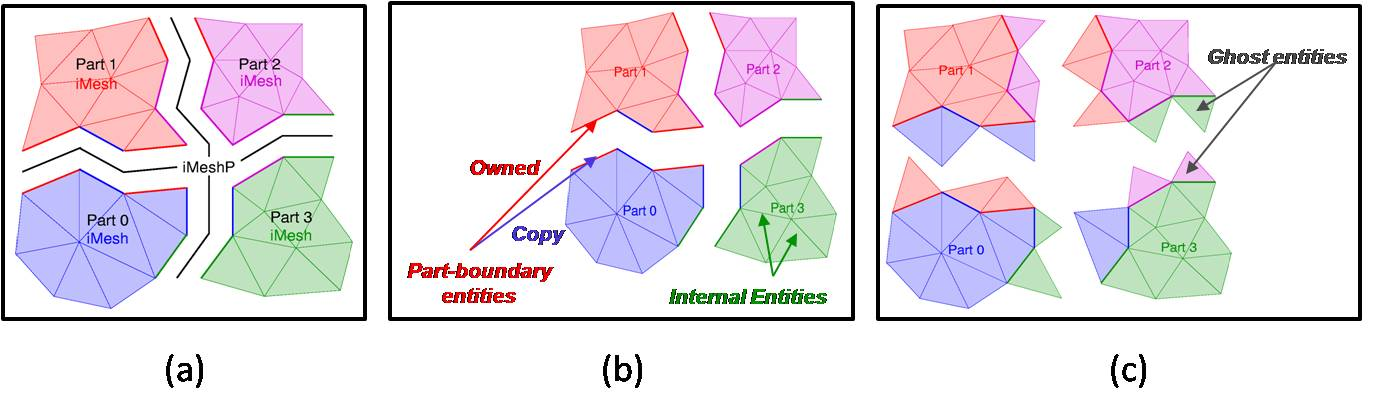
\includegraphics[height=1.75in]{Figures/imeshp.jpg}
\end{center}
\caption{A simple example showing the iMeshP datamodel.  Image (a) shows the relationship bewteen iMesh and iMeshP, (b) shows entity classification, and (c) shows ghost entities.}
\label{fig:data_model}
\end{figure}

\subsection{The ITAPS iMeshP Interface} 
\label{sec:interface}

Once the abstract data model is defined, the next step to creating
interoperable technologies is to define common interfaces that support
its functionality.  A key aspect of the ITAPS approach is that we do
not enforce any particular data structure or implementation with our
interfaces, requiring only that certain questions about the geometry,
mesh, or field data can be answered through calls to the
interface. All data passed through the interface is in the form of
opaque handles to objects defined in the data model.  One of the most
challenging aspects of this effort remains balancing performance of
the interface with the flexibility needed to support a wide variety of
data types.  Further challenges arise when considering the support of
many different scientific programming languages which we address using
a two-pronged approach.  First, we provide a C-language binding for
our interfaces that is compatible with most needs in scientific
computing.  Additional flexibility, albeit at a somewhat higher cost,
is supported through the use of the SIDL/Babel technology \cite{babel}
provided by the Common Component Architecture Forum.

In previous work, a full specification for the serial mesh interface,
called iMesh, was completed and implemented by several
institutions. The extension to iMeshP, the parallel mesh interface,
required the definition of a number of additional functions; for
example, functions to easily create and modify partitions, create
ghost entities, retrieve ghost and owner entity tag data, and
determine an entity's ownership status.  To simplify the iMeshP
interface, we allow part handles to be substituted for entity-set
handles in all serial iMesh functions.  Thus, operations such as
adding entities to parts and querying the number of entities in a part
can be achieved using the same interface as adding entities to and
querying entity sets.  Additional iMeshP functions provide information
about part boundaries and neighboring parts.  Furthermore, the iMeshP
interface supports parallel operations needed for efficient
computation, load balancing and mesh modification.  By necessity,
these operations involve parallel communication and both synchronous
and asynchronous parallel operations are supported. This design
enables such things as updates of tag data in ghost entities during
computation, large- or small-scale entity migration for dynamic load
balancing or edge swapping, updates of vertex coordinates in non-owned
vertices for mesh smoothing, and coordination in the creation of new
entities along part boundaries for mesh refinement.  For more
information see \cite{imeshp_web}.

To illustrate iMesh and iMeshP interface usage, we provide a simple
example of using the C-binding version in Figure \ref{fig:imesh}. Line
14 shows the creation of a new mesh instance which creates the local
opaque handle {\tt mesh} that is used in later calls to refer to this
instance of the interface on this process. Likewise, line 15 shows the
creation of the {\tt root\_set} which contains all the mesh data on
the processor once it is loaded.  Line 20 shows the call to create the
partition handle on all processors and associate the MPI communicator
with it.  Line 21 shows the use of the {\tt iMeshP\_load} function to
populate the mesh and partition interface on all processors using a string name
identifier.  In this example, the data is loaded from file {\tt
125hex.vtk}, but {\tt iMeshP\_load} can also be used for on-the-fly
mesh creation.  Line 24 shows the global query to retrieve the number
of parts in the partition.  Line 25 shows the call to get the global
number of vertices in the partition; this call may require global
communication if it is not stored locally.

\begin{figure}
\begin{small}
\begin{verbatim}
1  #include ``iMesh.h''
2  #include ``iMeshP.h''
4  #include <mpi.h>
5
6  int main( int argc, char *argv[] )
7  {
8      // create and populate the Mesh instance
9    iMesh_Instance mesh;
10   iBase_EntitySetHandle root_set;
11   iMeshP_PartitionHandle partition;
12   int num_parts, num_vtx, ierr;
13
14   iMesh_newMesh("", &mesh, &ierr, 0);
15   iMesh_getRootSet(mesh, &root_set, &ierr);
16
17   MPI_Init(&argc, &argv);
18
19    // create the partition and load the mesh
20   iMeshP_createPartitionAll(mesh, MPI_COMM_WORLD, &partition, &ierr)
21   iMeshP_load(mesh, partition, root_set, "125hex.vtk", "", &ierr, 10, 0);
22
23    // get the number of parts and number of vertices in the partition
24   iMeshP_getNumParts(mesh, partition, &num_parts, &ierr);
25   iMeshP_getNumOfTypeAll(mesh, partition, root_set, iBase_VERTEX, &num_vtx, &ierr); 
26 }
\end{verbatim}
\end{small}
\caption{Example use of the C-binding of the iMeshP interface.}\label{fig:imesh}
\end{figure}

\subsection{ITAPS Software Using iMesh and iMeshP}
\label{sec:software}

%\begin{itemize}
%
%\item The Flexible Mesh DataBase (FMDB) \cite{ReSh03,Seol06,Shep08} is designed
%especially to handle adaptively changing mesh data, including flexible
%storage of adjacency information.  It includes a complete iMesh
%implementation and a nearly complete iMeshP implementation. The FMDB
%implementation has been used to demonstrate mesh refinement from 17
%million elements to two billion elements on 32768 (32K) processors of an
%IBM Blue Gene/L computer. Application usage of FMDB includes computational
%fluid dynamics (CFD), fusion, and accelerator simulations.
%
%\item The Mesh Oriented datABase (MOAB) \cite{moab} is particularly
%%efficient in its memory management. MOAB has a complete implementation
%of iMesh and a partial implementation of iMeshP, using sets and tags
%to store and retrieve most parallel constructs in iMeshP.  Application
%usage for MOAB includes nuclear reactor modeling, neutron transport,
%and accelerator design optimization.
%
%\item The Generation and Refinement of Unstructured Mixed-element
%Meshes in Parallel (GRUMMP) \cite{GRUMMP:http} toolkit is particularly
%efficient in retrieving adjacency information.  Although designed
%primarily for triangular and tetrahedral mesh generation, improvement,
%and adaptation, GRUMMP supports all standard finite element
%topologies.  GRUMMP currently supports the iMesh interface, and
%support for iMeshP is planned.  Application usage is primarily in CFD,
%especially aerodynamics and non-Newtonian fluid dynamics.
%
%\item NWGRID \cite{nwgrid1,nwgrid2,nwgrid3} is intended for adaptive 
%mesh refinement, especially for simplicial meshes. The mesh generation
%capabilities supported by NWGrid include parallelized generation of
%large unstructured, hybrid meshes, adaptive mesh refinement, and
%swapping for simplicial meshes.  NWGrid is based on the Global Array
%paradigm and provides a complete iMesh implementation.  Application
%usage includes computational biology, CFD, solid mechanics, and
%subsurface transport modeling.
%
%\end{itemize} 
The ITAPS consortium has produced four implementations of the iMesh
interface based on pre-existing mesh databases.  Each of the four has
its own particular strengths and so are useful in different
application settings.  In addition, two of the four iMesh
implementations also have at least partial iMeshP implementations
available.  These implementations are listed in Table
\ref{tab:implementations}.  In addition, the ITAPS team is developing
a number of {\it component services} that use the iMesh and iMeshP
interfaces to support simulations involving complex domains, adaptive
techniques, and high-order methods.  Specific tools include mesh
quality improvement through smoothing with Mesquite
\cite{mesquite_download} and swapping \cite{frei-cfog:ijnme97},
high-order mesh curve correction tools \cite{Luo04}, adaptive mesh
refinement through MeshAdapt \cite{LiSh05}, front tracking through
FronTier \cite{BoFi07}, dynamic load balancing services through Zoltan
\cite{devi02}, and visualization plug-ins into VisIt
\cite{Childs:2005:ACS}. These component services can be used directly
by applications and can also be integrated to form higher-level
integrated services such as shape-optimization and AMR-Front tracking
technologies.  Each of these services has been demonstrated to work
with multiple implementations of the iMesh and iMeshP component APIs.
We generally see little reduction in the overall efficiency of an
application using the iMesh or iMeshP interfaces compared to using
native data structures when following the ITAPS ``best practices''
implementation guidelines.  For example, we tested the time to
partition a MOAB mesh using Zoltan through the MOAB native interfaces
and compared this with the time required to partition the same mesh
through the iMesh interface.  We found the overhead ranged from under
1\% for small problem sizes to about 2\% for larger problems sizes.
Similarly, when building a stiffness matrix associated with a simple
finite element solver, the overhead costs associated with the use of
iMesh ranged from 2\% to 11\% depending on the access pattern chosen.
\begin{table}[thbp]
\begin{center}
\caption{iMesh and iMeshP Implementations}
\label{tab:implementations}
\begin{small}

\begin{tabular}{|l|l|l|l|}
\hline
{\bf Implementation} & {\bf Emphasis}  & {\bf Parallel Capability} & {\bf Applicaitons} \\
\hline
FMDB: Flexible Mesh           & Adaptively changing      & Scalable to 32K & fusion, accelerators \\
Database \cite{ReSh03,Seol06} & meshes (entity addition  & procs; 2B elements & CFD, solid mechanics \\
(iMesh/iMeshP)         & or removal)                     &             & multiphase flow \\
\hline
MOAB: Mesh Oriented & Low memory usage & Up to 64 procs &  nuclear reactors, \\
dAtaBase \cite{moab}& first; then CPU  &                & accelerators, rad. \\
(iMesh/iMeshP)                    & time             &                & transport, inertial \\
 & & & confinement fusion\\
\hline
GRUMMP: Generation   & Fast adjacency retrieval & In development & CFD, biological \\
and Refinement of    & for mesh generation and  &  & systems, structural \\
Mixed-Element Meshes  & improvement, adaptation  &  & mechanics \\
in Parallel \cite{GRUMMP:http} (iMesh) & & & \\
\hline
NWGrid: Northwest & Simplicial meshes; &      Parallelism based &  CFD, subsurface \\
Grid Generation   & parallel generations of & on Global Arrays; & transport, biological \\
Code \cite{nwgrid3} (iMesh) & unstructured, hybrid, &   Scalable to at least & systems \\
                    & meshes &                  10K procs &  \\
\hline
\end{tabular}
\end{small}
\end{center}
\end{table}

%Many application users wishing to access ITAPS services will implement
%the ITAPS interfaces using their own mesh and geometry data
%structures.  Typically only a subset of the interface functions that
%%have been defined are needed to support each service.  For example, in
%Table \ref{tab:interface_calls} we show the number of entity access,
%modification, sets, tags, and parallel functions that need to be
%implemented to use the services mentioned above. To assist users
%developing implementations based on their own mesh data structures,
%the ITAPS team has developed a compliance test suite to ensure that
%interface definitions are properly interpreted and implemented.
%
%\begin{table}[htbp]
%\begin{center}
%\caption{Number of interface functions needed by the ITAPS services.}
%\label{tab:interface_calls}
%
%\begin{tabular}{|l|c|c|c|c|c|c|c|c|c|c|}
%\hline
% & \begin{sideways}Coordinates \end{sideways}
% & \begin{sideways}Adjacency \end{sideways}
% & \begin{sideways}Other queries \end{sideways}
% & \begin{sideways}Iterators \end{sideways}
% & \begin{sideways}Modification \end{sideways}
% & \begin{sideways}Basic Sets\end{sideways}
% & \begin{sideways}Tags \end{sideways}
% & \begin{sideways}Parallel \end{sideways}
% & \begin{sideways}iGeom/iRel \end{sideways}
% & \begin{sideways}Total \end{sideways} \\
%\hline
%Mesquite & 1 & 1 & 4 & 4 & 1 & 2 & 13 & & 6 & 13\\
%Swapping & 1 & 1 & 4 & 4 & 2 &   &    & &   & 12 \\ 
%MeshAdapt& 1 & 2 & 5 & 3 & 3 &   &  7 & 13 & & 34\\ 
%FronTier & 3 & 1 & 5 & 3 & 3 &   & 3  &    & & 18\\
%Zoltan   & 1 & 2 & 5 &   &   &   &    & 14 & & 22 \\ 
%VisIt    & 1 & 1 & 9 & 3 &   & 1 & 16 &    & & 31  \\
%\hline
%\end{tabular}
%\end{center}
%\end{table}

\section{Scalability of ITAPS software}
\label{sec:petascale}

In this section, we hightlight recent results on the scalability of
ITAPS tools that use the iMeshP interface.  In particular, in this
paper we focus on the combintation of the FMDB mesh database, 
Zoltan dynamic load balancing, and MeshAdapt services used in implicit
finite element and finite volume applications.  We are interested in
both strong and weak scaling to minimize run time and maximize
resolution, respectively. This has driven the need to research new
load balancing technologies and communication tools; particularly as we
scale to O(100,000) processors and beyond.  We describe these research
efforts in some detail and highlight the resulting scalability of our
tools and solvers that use our tools on a number of different
leadership class computers.

The ability to scale implicit finite element and finite volume
computations such as those used in the accelerator and fusion SciDAC
application efforts, requires ensuring both the system formulation and
solution are effectively load balanced. Graph-based partitioners are
well known to produce a partitioning of the mesh into parts that are
well balanced in terms of the specified partition object type while
also minimizing inter-part communications. However, traditional
graph-partitioners consider a single objective optimization subject to
a single balance constraint. In the case of mesh-based analysis, the
defined graph nodes are often mesh regions. This selection does an
excellent job of balancing the number of regions (elements) and
therefore the workload for the construction of the part-level finite
element system. However, in the case of $C^0$ interpolating basis
functions, for example, the workload balance for the iterative
solution (e.g. matrix vector product and vector norms) of the
resulting system is proportional to the number of mesh vertices per
part. Since mesh vertices are not the objects in the original
partitioning, the balance may not be optimal, particularly when the
numbers of mesh entities per part is relatively low (e.g., a few
thousand). We are developing two multiple compute-object based
partition improvement algorithms to reduce the vertex imbalance
thereby improving the overall balance of two mesh entities as required
by a scalable implicit solve. They are referred to as local iterative
inter-part boundary modification (LIIPBMod) and heavy part split
(HPS).

\begin{itemize}
\item {\it The LIIPBMod Algorithm.}  LIIPBMod locally migrates small numbers
of mesh regions from parts that are relatively heavily loaded with
respect to mesh vertices to neighboring parts which are relatively
lightly loaded with respect to mesh entities. On the heavily loaded
part, the mesh vertices on the part boundary are traversed and the
ones bounding a small number of elements are identified. If the
neighboring part is lightly loaded, the whole ``cavity'' (all the
adjacent elements of the picked vertex) is migrated to the neighboring
part. By this minor inter-part boundary adjustment, the vertex
imbalance is improved while only modestly perturbing the good element
balance. This procedure may need to be repeated for several iterations
to achieve desired vertex balance.

\item {\it The HPS Algorithm,} Our studies of the mesh partitions given by a
graph-based partitioner show that the percentage of heavily loaded parts
(more than 10\% imbalance) is usually less than 1\%. The idea of HPS
is that, if the desired number of parts is numP, first distribute the
mesh to 99\%*numP parts by a graph-based partitioner and leave the
other 1\%*numP parts empty. Then, select the 1\%*numP parts with the
highest vertex load and split them into two parts (i.e. migrate
roughly half of the mesh entities from them to one of the empty
parts). The splitting makes the heavily loaded parts become lightly
loaded. Since the peak of the imbalance determines the scalability,
HPS lowers the peak and hence improves the performance. 
%Figure \ref{fig:HPS} illustrates this algorithm using a 16 part example.
\end{itemize}
%
%\begin{figure}[htb] 
%\begin{center}
%\includegraphics[height=1.5in]{Figures/HPS.png}
%\end{center}
%\caption{Vertex imbalance before and after HPS.  The partitions on parts 1 and 7 are split and given to parts 15 and 16 to improve overall performance.}
%\label{fig:HPS}
%\end{figure}

Figure \ref{fig:LIIP_HPScompare} shows the results of applying the
two algorithms to a 16.7M element anisotropically adapted mesh used in
the simulation of an abdominal aorta aneurism (left image). The two
graphs (center for LIIPBmod and right graph for HPS) indicate the
number of vertices per part divided by the average per part
before (red dots) and after (blue dots) application of the
algorithms. Note in both cases the spikes (red dots in the upper parts
of the graphs) that reduce scalability are dramatically lowered after
the algorithms have been applied.

\begin{figure}[htb] 
\begin{center}
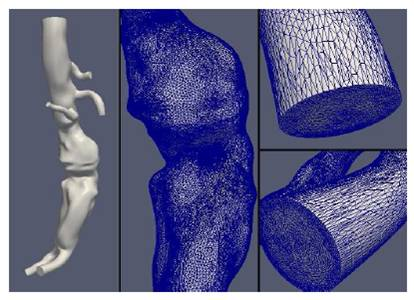
\includegraphics[height=1.35in]{Figures/AAA.jpg}
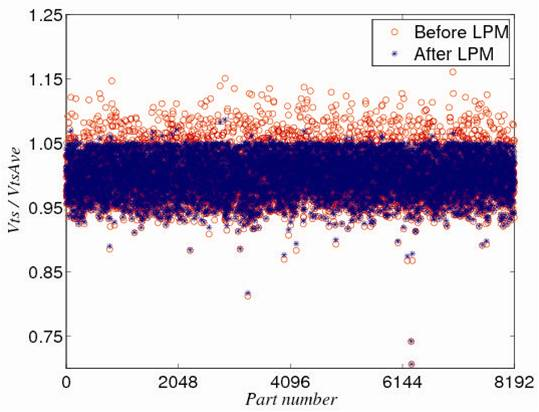
\includegraphics[height=1.5in]{Figures/LIIPBMod8192.jpg}
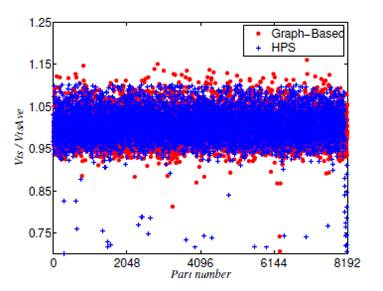
\includegraphics[height=1.5in]{Figures/HPS8192.jpg}
\end{center}
\caption{Vertex imbalance before and after LIIPBMod and HPS.}
\label{fig:LIIP_HPScompare}
\end{figure}

Using the results of the multi-compute object load balancer, we
showed that unstructured mesh solvers based on implicit methods can
scale to very large numbers of processors \cite{Shep07}.  Table
\ref{tab:scaling} illustrates the parallel efficiency of PHASTA, a parallel,
unstructured and implicit flow solver developed at RPI on up to
O(100,000) cores of IBM BG and Cray XT systems \cite{phasta}.  PHASTA
uses FMDB and the MeshAdapt service for refinement on up to 32K
processors and iMeshP and iZoltan to partition the resulting meshes
into 128K parts for distribution to almost the full machine for the analysis
step.  Near-perfect (linear) strong scaling of the analysis step over
multiple doublings of cores can be clearly seen on various systems
with a slight decrease in parallel efficiency on the largest core
counts due to the fact that computational load per core becomes
insignificant (for a fixed-size problem).  More information on PHASTA's
scaling studies can be found in \cite{SaCa09}.

\begin{table}[htbp]
\begin{center}
\caption{Strong scaling results of PHASTA up to O(100,000) cores on IBM BlueGene (BG)
and Cray XT systems (1 implies perfect scaling with 100\% parallel efficiency)}.
\label{tab:scaling}
\begin{footnotesize}
\begin{tabular}{|l|l|l|l|c|l|l|}
\cline{1-4}  
\cline{6-7}
\multicolumn{4}{|c|}{\bf 105 Million Elements} & &
\multicolumn{2}{|c|}{\bf 1 Billion Elements} \\
%\multicolumn{4}{|c|}{\cline{1-4}} & & \multicolumn{2}{|c|}{\cline} \\
\cline{1-4}  
\cline{6-7}
Core &  BGL-CCNI  & BGP-ALCF & XT4-NERSC&  &  Core &   BGP-ALCF \\
Count  & \multicolumn{1}{|c|}{RPI} & \multicolumn{1}{|c|}{ANL} &     \multicolumn{1}{|c|}{LBNL} &       &  Count   & \multicolumn{1}{|c|}{ANL} \\
\cline{1-4}  
\cline{6-7}
512    &   	1.00   &       	1.00 &    1.00   & &  16,384   &	1.00 \\
1,024  & 	1.01   &       	1.02 &    1.03   & &  32,678   &	0.99  \\
2,048  &	1.00   &       	0.99 &    1.16   & &  65,536   &	0.97 \\
4,096  &  	0.99   &       	0.99 &    1.00   & &  131,072  & 	0.89 \\
\cline{6-7}
8,192  & 	1.02   &       	0.95 &    0.77   &  \multicolumn{3}{c}{}  \\
16,384 &	1.03   &       	0.95 &           &  \multicolumn{3}{c}{}  \\
32,768 & 	0.93   &       	0.88 &           &  \multicolumn{3}{c}{}  \\
\cline{1-4}  
\end{tabular}
\end{footnotesize}
\end{center}
\end{table}

We have also examined the scaling of the MeshAdapt service in both the
weak and strong sense.  Mesh adaptation is characterized by small, but
variable, work per operation which implies that achieving ``perfect
scaling'' can be very costly.  In particular, our research has found that
we can run adaptive mesh refinement algorithms on the large numbers of
parts typically used in a simulation analysis, and the overall time
will still be a small percentage of the overall total solution time.
For example, for the weak scaling results shown in Table
\ref{tab:refinement_scaling} for uniform adaptive refinement, the time 
required by the adaptivity algorithms for the largest case on 32768
processors is only 0.04\% of the total time.

That said, the scaling efficiency is clearly decreasing as the number
of processors increases, and to improve the scaling characteristics of
the MeshAdapt and other services, we are developing a new general-purpose,
MPI-based communication package called the Inter-Processor
Communication Manager (IPComMan).  This package aims to reduce data
exchange costs by exploiting communications in a local neighborhood
for each processor. The neighborhood is the subset of processors
exchanging messages with each other during a specific communication
round, which in many applications is bounded by a constant, typically
under 40, independent of the total number of processors. 
%The basic
%idea of the library is to keep the message-passing within subdomains,
%and eliminate, or reduce, the number of collective calls needed.  
%We note that there are situations when it is
%not possible to a priori define all the neighbors for processors,
%i.e., new neighbors may be encountered during a mesh modification step. As
%new neighbors needing to communicate will be unaware of each other,
%one collective call at the end of the communication round is performed
%to support neighborhood changes.  
%The library provides several useful features including: i) automatic
%message packing, ii) management of sends and receives with
%non-blocking MPI functions, iii) asynchronous behavior unless the
%other is specified, and iv) support of dynamically changing
%neighborhoods during communication steps.
Strong scaling of uniform adaptive mesh refinement using the IPComMan
Message Passing library for a mesh starting with 4.3M elements and
ending with 2.2B elements is shown in the right of Table
\ref{tab:refinement_scaling}.  Significant improvements in scaling efficiency
compared to the weak scaling case are evident due to decreased communication
costs.

\begin{table}[htbp]
\begin{center}
\caption{Uniform adaptive mesh refinement: weak scaling using the AutoPack Message Passing library and strong scaling using the IPComMan library}
\label{tab:refinement_scaling}
\begin{tabular}{|c|c|c|c|c|c|c|c|c|}
\cline{1-5}  
\cline{7-9}
\multicolumn{5}{|c|}{\bf Weak Scaling} & &
\multicolumn{3}{|c|}{\bf Strong Scaling} \\
\cline{1-5}  
\cline{7-9}
Number of & Initial & Adapted & Time & Scaling & & Number of & Time &
Scaling \\ 
Parts & Mesh & Mesh & (s) & Factor & &  Parts & (s) & Factor\\
\cline{1-5}  
\cline{7-9}
2048 & 17M & 128M & 5.0 & 1.0 & & 
2048 & 21.5 & 1.0 \\
4096 & 34M & 274M & 4.8 & 1.05 & &
4096 & 11.2 & 0.96 \\
8192 & 65M & 520M & 5.1 & 0.97 & &
8192 & 5.67 & 0.95\\
16384 & 520M & 1.1B & 6.1 & 0.82& &
16384 & 2.73 & 0.99\\
\cline{7-9}
32768 & 274M & 2.2B & 7.4 & 0.68 &   \multicolumn{4}{c}{}  \\
\cline{1-5}
\end{tabular}
\end{center}
\end{table}

\section{Use of ITAPS Parallel Adaptive Software in SciDAC Applications}
\label{sec:application}

ITAPS technologies have impacted DOE applications in a number of ways
including direct use of the services and software described in this
paper (adaptive algorithms, mesh quality improvement, partitioning,
front tracking), technology advancement through the demonstration and
insertion of key new technology areas (shape optimization and
petascale mesh generation), and by looking ahead and anticipating the
needs of application teams through the development of new services
(mesh to mesh transfer for coupling multiphysics applications).  In
this section we highlight a few key examples of the use of ITAPS
software in SciDAC applications.  While we focus on our interactions
with accelerator and fusion applications to insert adaptivity into
their codes in this paper, more extensive interactions funded under
the auspices of the SciDAC and other DOE programs include work with
multiple accelerator and fusion teams along with subsurface flow and
nuclear energy application teams.

{\it Accelerator Design.} The ITAPS team is working extensively with
the ``Community Petascale Project for Accelerator Science and
Simulation (COMPASS)'' SciDAC project, and in particular researchers
at the SLAC National Accelerator Laboratory, to provide high-order
mesh generation and adaptive control methods to improve the processes
for the design and optimization of accelerator cavities. For example,
in calculating the short-range wakefield inside an accelerator
structure, only the small region in the vicinity of the moving
particle beam is required to have a highly refined mesh in the
simulation. The moving curved mesh adaptation procedure, which refines
a small region of interest near the beam (see Figure
\ref{fig:moving_mesh}), greatly reduces the computational effort
required for a given level of accuracy.  In particular, using such
techniques has resulted in a tenfold reduction in the computational
cost of these simulations \cite{luo08a, lee08}.

\begin{figure}[tbhp]
\centering
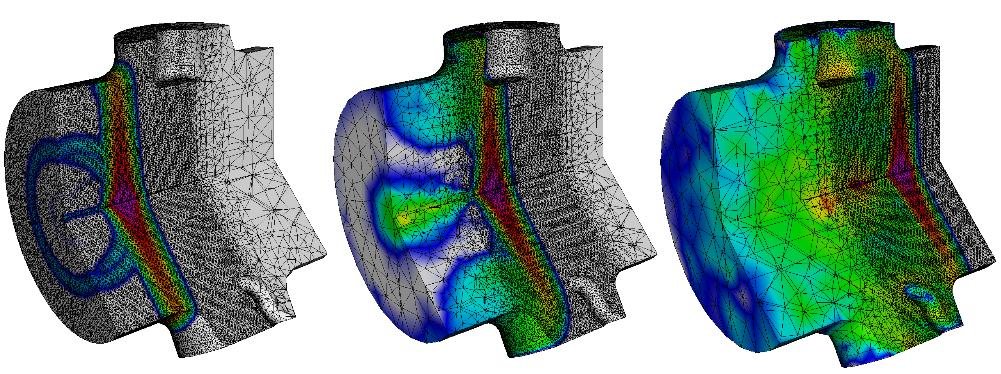
\includegraphics[width=4.5in]{Figures/moving.jpg}
\caption{\label{fig:moving_mesh} The electric fields on tree-refined curved 
meshes around the moving beam}
\end{figure}

{\it Fusion.} The SciDAC-funded ``Center for Extended MHD modeling
(CEMM)'' has extensively used a 3D MHD code to simulate global
instabilities in magnetic fusion devices.  The ITAPS team is working
with CEMM fusion scientists to extend the MHD high-order finite
element software (M3D-C1) to interface with unstructured mesh
adaptation technologies. This enables them to gain the efficiencies of
using adaptive meshes (see Figure \ref{fig:fusion_mesh} for isotropic
and anisotropic adapted meshes \cite{Jard07,jard08}) and allows them
to model general curved reactor domains (see the rightmost image in
Figure \ref{fig:fusion_mesh}). 
\begin{figure}[htbp]
\centering
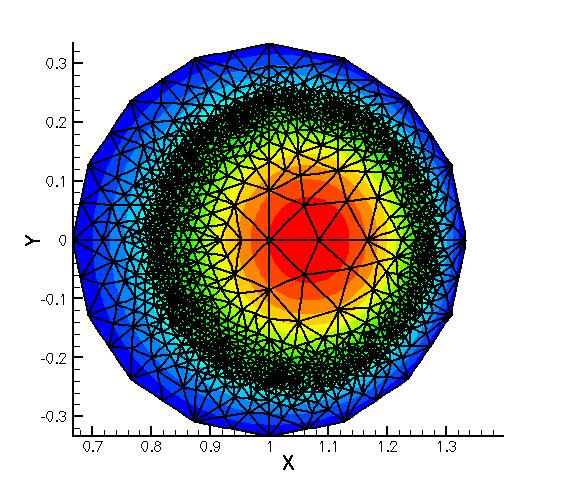
\includegraphics[width=1.75in]{Figures/adapted.jpg}
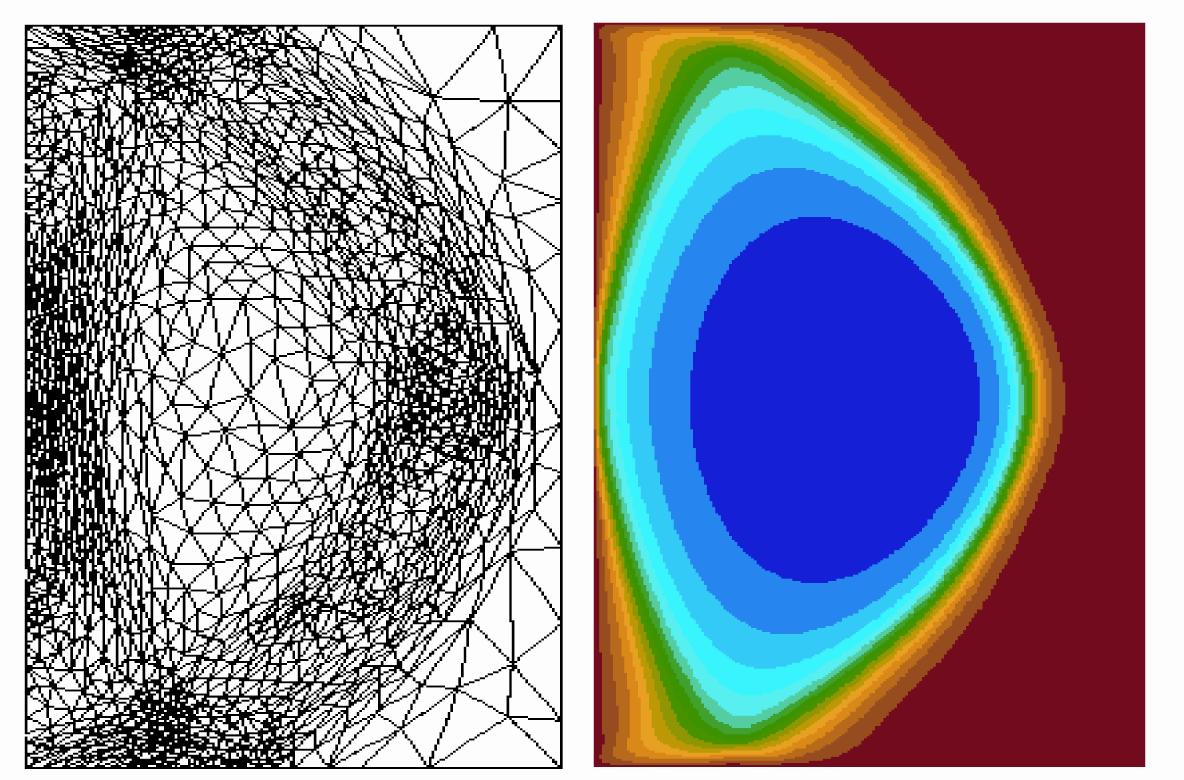
\includegraphics[width=2.25in]{Figures/anisotropic.jpg}
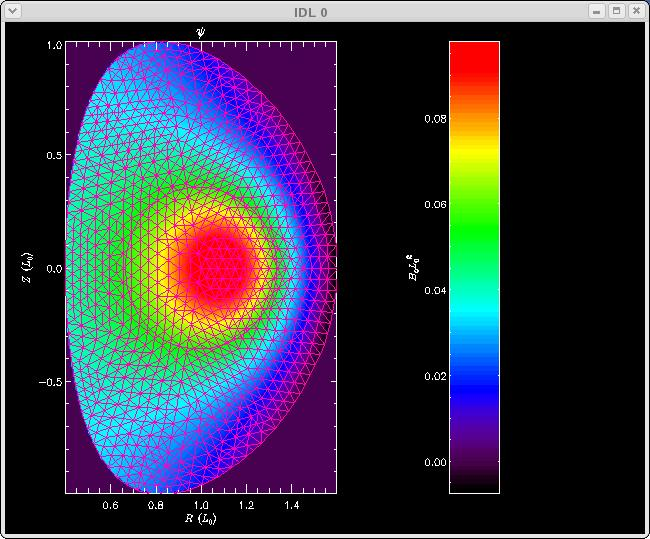
\includegraphics[width=1.75in]{Figures/PPPL-CURVED.jpg}
\caption{\label{fig:fusion_mesh} Isotropic and anisotropic mesh adaptation to
increase computational efficiency in fusion applications.
On the far right we show the vorticity contours in a 
curved reactor domain.}
\end{figure}

\section*{More Information about ITAPS}
More information on the ITAPS project including detailed descriptions
of the ITAPS services, interfaces, software, and interactions with SciDAC
application teams can be found at \url{http://www.itaps-scidac.org}.

\ack
This work was performed under the auspices of the U.S. Department of
Energy by Lawrence Livermore National Laboratory under Contract
DE-AC52-07NA27344; the Canadian Natural Sciences and Engineering
Research Council under Special Research Opportunities Grant
SRO-299160; by Rensselaer Polytechnic Institute under DOE grant number
DE-FC02-01ER25460 and the NSF PetaApps project OCI-0749152, and by
Sandia National Laboratory; a multiprogram laboratory operated by
Sandia Corporation, a Lockheed Martin Company, for the U. S.
Department of Energy's National Nuclear Security Administration under
contract DE-AC04-94AL85000.  Computing Resources used in this paper
include the Rensselaer Computational Center for Nanotechnology
Innovations (BG/L) and DOE INCITE (Intrepid - BG/P).

\section*{References}
\bibliographystyle{iopart-num}
\bibliography{itaps}


\end{document}
